\documentclass[11pt,a4paper]{article}

% Packages
\usepackage{times}
\usepackage{url}
\usepackage{latexsym}
\usepackage{amsmath,amssymb}
\usepackage{graphicx}
\usepackage{booktabs}
\usepackage{algorithm}
\usepackage[noend]{algorithmic}
\usepackage{hyperref}
\usepackage{geometry}
\usepackage{tocbibind}
\usepackage{natbib}
\geometry{margin=1in}

% Custom commands
\newcommand{\cudos}{CUDOS}
\newcommand{\rag}{RAG}
\newcommand{\dea}{DEA}
\newcommand{\subagent}{sub-agent}
\newcommand{\subagents}{sub-agents}

% Title
\title{Retrieval-Driven Self-Improvement: A Multi-Agent Architecture for Theory-Grounded Academic Review}

% Authors
\author{
\begin{minipage}[t]{0.45\textwidth}
\centering
Yu Yang$^{1}$\\
\vspace{0.2em} 
\small $^{1}$Dongbi Scientific Data Lab, Beijing, China\\
\vspace{0.1em} 
\small \texttt{yuyang@dongbidata.com}
\end{minipage}
\hfill
\begin{minipage}[t]{0.45\textwidth}
\centering
Dengsheng Wu$^{2}$\\
\vspace{0.2em} 
\small $^{2}$Shenzhen University, Shenzhen, China
\end{minipage}
\\[1em]  
\begin{minipage}[t]{0.45\textwidth}
\centering
Xing Wei$^{3}$\\
\vspace{0.2em} 
\small $^{3}$Dongbi Scientific Data Lab, Beijing, China
\end{minipage}
}

\date{\today}

\begin{document}

\maketitle

\begin{abstract}
Peer review is the cornerstone of scientific progress, yet traditional peer review faces challenges of inefficiency, inconsistent standards, and subjective evaluation. While AI-assisted review tools have emerged, they predominantly operate at the ``technical'' level, lacking theoretical foundations from the philosophy of science. More critically, existing tools treat knowledge bases as static, failing to adapt to evolving disciplinary standards and reviewer feedback. In this paper, we present WuYa, a theory-driven multi-agent system that transforms classical philosophical principles into an operational architecture for academic paper evaluation. WuYa introduces five key innovations: (1) a retrieval-evaluation coupling mechanism where \rag{} serves as the core triggering mechanism for judgment; (2) a two-phase routing architecture with CUDOS gatekeeping and parallel expert evaluation; (3) a hybrid knowledge strategy combining prompt-internalized ``principles'' with \rag{}-retrieved ``evidence''; (4) an LLM-as-mapper approach with discipline prior calibration for paper localization; and (5) a self-improving frontier discovery mechanism that learns evaluation preferences from editor feedback. Experiments on 5,000 papers across five disciplines demonstrate that WuYa achieves 70.3\% top-5 recommendation accuracy and 0.72 Spearman correlation with human experts.
\end{abstract}

\section{Introduction}
\label{sec:introduction}

Peer review is the cornerstone of scientific progress, serving as the primary mechanism for quality assurance, knowledge dissemination, and scholarly communication. Yet the traditional peer review system faces mounting challenges: reviewer shortages, inconsistent standards, lengthy turnaround times, and subjective evaluation criteria \citep{smith2006peer}.

Recent advances in artificial intelligence have spawned a new generation of AI-assisted review tools. These systems can identify methodological flaws, check statistical assumptions, and even generate review reports \citep{liu2023review}. However, most existing tools operate at the ``technical'' level, focusing on surface features like grammar, formatting, and basic statistical checks. They lack theoretical foundations from the philosophy of science---the very disciplines that have spent decades studying how knowledge is created, validated, and transmitted.

More critically, existing systems treat knowledge bases as static. They do not learn from reviewer feedback, adapt to evolving disciplinary standards, or capture journal-specific evaluation preferences. This static approach is ill-suited to the dynamic nature of academic research, where standards evolve and journals develop distinct editorial identities.

In this paper, we present \textbf{WuYa} (In Chinese meaning ``boundless''), a theory-driven multi-agent system that transforms classical philosophical principles into an operational architecture for academic paper evaluation. WuYa addresses the limitations of existing tools through five key innovations:

\begin{enumerate}
    \item \textbf{Retrieval-Evaluation Coupling}: Unlike systems that treat retrieval as supplementary, WuYa makes \rag{} the core triggering mechanism for evaluation. Retrieved canonical texts are not merely cited---they actively shape the evaluation criteria and reasoning process.
    
    \item \textbf{Two-Phase Routing}: WuYa separates normative gatekeeping (CUDOS norms) from substantive evaluation (Innovation, Method, Evidence, Application). This architecture ensures that ethical considerations are addressed before quality assessment.
    
    \item \textbf{Hybrid Knowledge Strategy}: WuYa combines prompt-internalized ``principles'' (the ``dao'') with \rag{}-retrieved ``evidence'' (the ``shu''). This dual strategy balances consistency and flexibility.
    
    \item \textbf{LLM-as-Mapper with Discipline Priors}: For paper-to-journal matching, WuYa uses LLMs as cross-disciplinary mappers, calibrated by empirical prior distributions from citation network analysis.
    
    \item \textbf{Self-Improving Frontier Discovery}: WuYa learns from editor feedback through a frontier discovery mechanism that captures and accumulates evaluation preferences over time.
\end{enumerate}

Our experiments on 5,000 papers across five disciplines demonstrate that WuYa achieves 70.3\% top-5 recommendation accuracy and 0.72 Spearman correlation with human expert ratings, significantly outperforming existing baselines.

\section{Related Work}
\label{sec:related-work}

\subsection{AI-Assisted Peer Review}

The application of AI to peer review has gained significant attention. Early systems focused on surface-level checks: plagiarism detection \citep{mozgovoy2020automatic}, statistical assumption validation \citep{nuijten2016prevalence}, and basic grammar correction. More recent systems attempt deeper analysis: PaperDigest \citep{kang2018peerread} extracts key claims and evidence, while ReviewAdvisor \citep{yuan2022reviewadvisor} generates review comments based on paper content.

However, these systems share a common limitation: they operate without theoretical grounding in the philosophy of science. They can identify \textit{that} a method is flawed but cannot explain \textit{why} it matters in terms of scientific validity or epistemic contribution.

\subsection{Multi-Agent Systems for Evaluation}

Multi-agent architectures have shown promise for complex evaluation tasks. \citet{du2023improving} demonstrate that multiple specialized agents can outperform monolithic systems through division of labor. \citet{liang2024encouraging} show that agent debate improves reasoning quality.

WuYa extends this approach by assigning each agent a specific philosophical foundation. The Innovation Sub-agent draws on Kuhn and Schumpeter; the Method Sub-agent on Pearl and Campbell; the Evidence Sub-agent on Popper and Lakatos; and the Application Sub-agent on Bush and Mokyr.

\subsection{Retrieval-Augmented Generation}

\rag{} has become a standard technique for grounding LLM outputs in external knowledge \citep{lewis2020retrieval}. In academic contexts, \rag{} has been used for literature review generation \citep{shah2023ai} and citation recommendation \citep{zhang2023citation}.

WuYa's innovation is to make retrieval the \textit{triggering mechanism} for evaluation rather than merely a citation source. Retrieved canonical texts determine which evaluation criteria are activated and how they are weighted.

\subsection{Self-Improving Agents}

Recent work has explored agents that improve through interaction. Reflexion \citep{shinn2023reflexion} uses verbal reinforcement learning to help agents learn from failures. Voyager \citep{wang2023voyager} builds a skill library through embodied exploration in Minecraft. These systems demonstrate that agents can learn from feedback and accumulate knowledge over time.

WuYa adapts these principles to the domain of academic evaluation. The Frontier Discovery Sub-agent learns from editor/reviewer feedback, building a library of ``frontier surfaces'' that capture evaluation preferences.

\subsection{Data Envelopment Analysis in Research Evaluation}

\dea{} has been applied to research evaluation, primarily for ranking research units \citep{johnes2006data} and assessing research efficiency \citep{cherchye2004scientific}. WuYa is the first system to integrate \dea{} into an agent-based paper evaluation workflow, using it as Path B for paper localization.

\subsection{Comparison with Existing Frameworks}

Table~\ref{tab:comparison} summarizes how WuYa differs from existing approaches.

\begin{table}[t]
\centering
\caption{Comparison of WuYa with Existing Approaches}
\label{tab:comparison}
\begin{tabular}{@{}lcccc@{}}
\toprule
\textbf{Feature} & \textbf{PaperDigest} & \textbf{ReviewAdvisor} & \textbf{Reflexion} & \textbf{WuYa} \\
\midrule
Theory Grounding & None & None & N/A & Philosophy of Science \\
Multi-Agent & No & No & Yes & Yes (5 specialized) \\
RAG Integration & No & Limited & No & Core mechanism \\
Self-Improvement & No & No & Yes & Frontier Discovery \\
DEA Analysis & No & No & No & Yes \\
\bottomrule
\end{tabular}
\end{table}

\section{Theoretical Foundations}
\label{sec:theory}

WuYa's architecture is grounded in classical theories from the philosophy of science. Each evaluation dimension maps to a distinct theoretical tradition, ensuring that judgments are not merely technical but epistemically principled.

\subsection{Innovation: Kuhn and the Nature of Scientific Change}

Thomas Kuhn's \textit{Structure of Scientific Revolutions} \citep{kuhn1962structure} provides the foundation for evaluating innovation. Kuhn distinguished between ``normal science'' (incremental progress within an existing paradigm) and ``revolutionary science'' (paradigm shifts that transform a field).

The Innovation Sub-agent applies this framework by assessing:
\begin{itemize}
    \item \textbf{Novelty level}: Does the paper operate within the current paradigm or challenge it?
    \item \textbf{Knowledge bridging}: Does it connect different paradigms or knowledge domains?
\end{itemize}

We also draw on Schumpeter's concept of ``creative destruction'' \citep{schumpeter1942capitalism} and Mokyr's distinction between ``Q-knowledge'' (knowing what) and ``A-knowledge'' (knowing how) \citep{mokyr2002gifts}.

\subsection{Method: Pearl and the Ladder of Causation}

Judea Pearl's \textit{Ladder of Causation} \citep{pearl2018book} provides the framework for method evaluation. The three rungs---association, intervention, and counterfactuals---offer a hierarchy of methodological sophistication.

The Method Sub-agent evaluates:
\begin{itemize}
    \item \textbf{Causal level}: Does the paper claim causal relationships? If so, at what rung?
    \item \textbf{Internal validity}: Are confounders adequately addressed?
    \item \textbf{External validity}: Can findings generalize beyond the study context?
\end{itemize}

We supplement Pearl with Donald Campbell's work on quasi-experimental designs \citep{campbell1963experimental} and Fisher's foundational work on statistical inference.

\subsection{Evidence: Popper, Lakatos, and Falsification}

Karl Popper's falsificationism \citep{popper1934logic} and Imre Lakatos's methodology of scientific research programmes \citep{lakatos1970falsification} inform the Evidence Sub-agent.

Key evaluation criteria include:
\begin{itemize}
    \item \textbf{Falsifiability}: Are claims testable? Are null results possible?
    \item \textbf{Evidence strength}: Is the evidence consistent with the claims? Does it rule out alternatives?
    \item \textbf{Replicability}: Can the study be reproduced?
\end{itemize}

\subsection{Application: Bush, Mokyr, and the Innovation Pipeline}

Vannevar Bush's linear model of innovation \citep{bush1945science} and Mokyr's framework for knowledge transfer \citep{mokyr2002gifts} guide the Application Sub-agent.

Evaluation focuses on:
\begin{itemize}
    \item \textbf{Technology Readiness Level (TRL)}: How close is the research to practical application?
    \item \textbf{Translation path}: Is there a clear path from research to impact?
    \item \textbf{Feedback mechanisms}: Does the research incorporate real-world feedback?
\end{itemize}

\subsection{CUDOS: Merton and the Norms of Science}

Robert Merton's CUDOS norms \citep{merton1942normative}---Communalism, Universalism, Disinterestedness, and Organized Skepticism---provide the foundation for normative evaluation.

The CUDOS Sub-agent serves as a gatekeeper, evaluating:
\begin{itemize}
    \item \textbf{Communalism}: Is knowledge shared openly? Are data and code available?
    \item \textbf{Universalism}: Are claims evaluated by objective criteria rather than personal attributes?
    \item \textbf{Disinterestedness}: Are there conflicts of interest?
    \item \textbf{Organized Skepticism}: Does the paper acknowledge limitations?
\end{itemize}

Papers that fail CUDOS evaluation are ``vetoed'' before substantive evaluation proceeds.

\subsection{Summary: From Theory to Operation}

Table~\ref{tab:theory-mapping} summarizes the theoretical foundations and their operationalization.

\begin{table}[t]
\centering
\caption{Theoretical Foundations and Operational Criteria}
\label{tab:theory-mapping}
\begin{tabular}{@{}llll@{}}
\toprule
\textbf{Dimension} & \textbf{Primary Theorists} & \textbf{Key Concepts} & \textbf{Criteria} \\
\midrule
Innovation & Kuhn, Schumpeter, Mokyr & Paradigm shift, Creative destruction & Novelty, Bridging \\
Method & Pearl, Campbell, Fisher & Causal ladder, Validity & Causal level, Rigor \\
Evidence & Popper, Lakatos & Falsification, Research programmes & Testability, Strength \\
Application & Bush, Mokyr & Innovation pipeline, TRL & Readiness, Translation \\
CUDOS & Merton & Scientific norms & Communalism, Skepticism \\
\bottomrule
\end{tabular}
\end{table}

\section{System Architecture}
\label{sec:architecture}

WuYa is organized as a multi-agent system with a central Router coordinating specialized Sub-agents. The architecture follows a two-phase routing design with retrieval-evaluation coupling.

\subsection{Overview}

The system workflow comprises:
\begin{enumerate}
    \item \textbf{Input}: Paper (PDF or text) + User intent (recommendation or review).
    \item \textbf{Phase 1}: CUDOS Sub-agent performs normative gatekeeping.
    \item \textbf{Phase 2}: Four evaluation Sub-agents (Innovation, Method, Evidence, Application) execute in parallel.
    \item \textbf{Aggregation}: Router combines scores into a five-dimensional vector.
    \item \textbf{Localization}: Path A (LLM-as-Mapper) and/or Path B (DEA) estimate paper tier.
    \item \textbf{Output}: Recommendation list or review report with RAG-grounded explanations.
\end{enumerate}

\subsection{Two-Phase Routing}

\subsubsection{Phase 1: CUDOS Gatekeeping}

The CUDOS Sub-agent evaluates the paper against Merton's norms. If any norm is violated (e.g., data withholding, undisclosed conflicts), the paper is ``vetoed'' and a veto report is generated. This ensures that ethical considerations are addressed before quality assessment.

\subsubsection{Phase 2: Parallel Evaluation}

If the paper passes CUDOS gatekeeping, the Router spawns four evaluation Sub-agents in parallel. Each Sub-agent:
\begin{enumerate}
    \item Analyzes the paper through its specialized theoretical lens.
    \item Generates scores (1-5) on its dimension's sub-criteria.
    \item Triggers RAG retrieval when criteria are ambiguous or contested.
    \item Produces a narrative explanation grounded in canonical texts.
\end{enumerate}

\subsection{Retrieval-Evaluation Coupling}

A key innovation of WuYa is that retrieval is not merely supplementary but serves as the \textit{triggering mechanism} for evaluation. The RAG layer indexes canonical texts organized by theorist and concept:

\begin{itemize}
    \item \textbf{Primary sources}: Full texts of Popper, Kuhn, Lakatos, Merton, Fisher, Campbell, Pearl, Bush, Mokyr.
    \item \textbf{Secondary sources}: Commentary and application of these theories.
    \item \textbf{Trigger logic}: Sub-agents invoke RAG when confidence is low or criteria are contested.
\end{itemize}

Retrieved passages are not merely cited---they actively shape the evaluation. For example, if the Method Sub-agent retrieves Pearl's discussion of the ``causal ladder,'' it will evaluate the paper's causal claims against that framework.

\subsection{Hybrid Knowledge Strategy}

WuYa employs a hybrid knowledge strategy inspired by the Chinese philosophical distinction between ``dao'' (principle) and ``shu'' (technique):

\begin{itemize}
    \item \textbf{Dao (Internalized)}: Core theoretical principles are internalized in Sub-agent prompts. This ensures consistency and reduces retrieval latency for standard cases.
    \item \textbf{Shu (Retrieved)}: Specific evidence and nuanced arguments are retrieved from the canonical corpus. This provides flexibility and grounding for edge cases.
\end{itemize}

The balance is dynamically adjusted: common scenarios rely primarily on internalized knowledge, while ambiguous cases trigger heavier retrieval.

\subsection{System Diagram}

Figure~\ref{fig:architecture} illustrates the WuYa system architecture.

\begin{figure}[t]
    \centering
    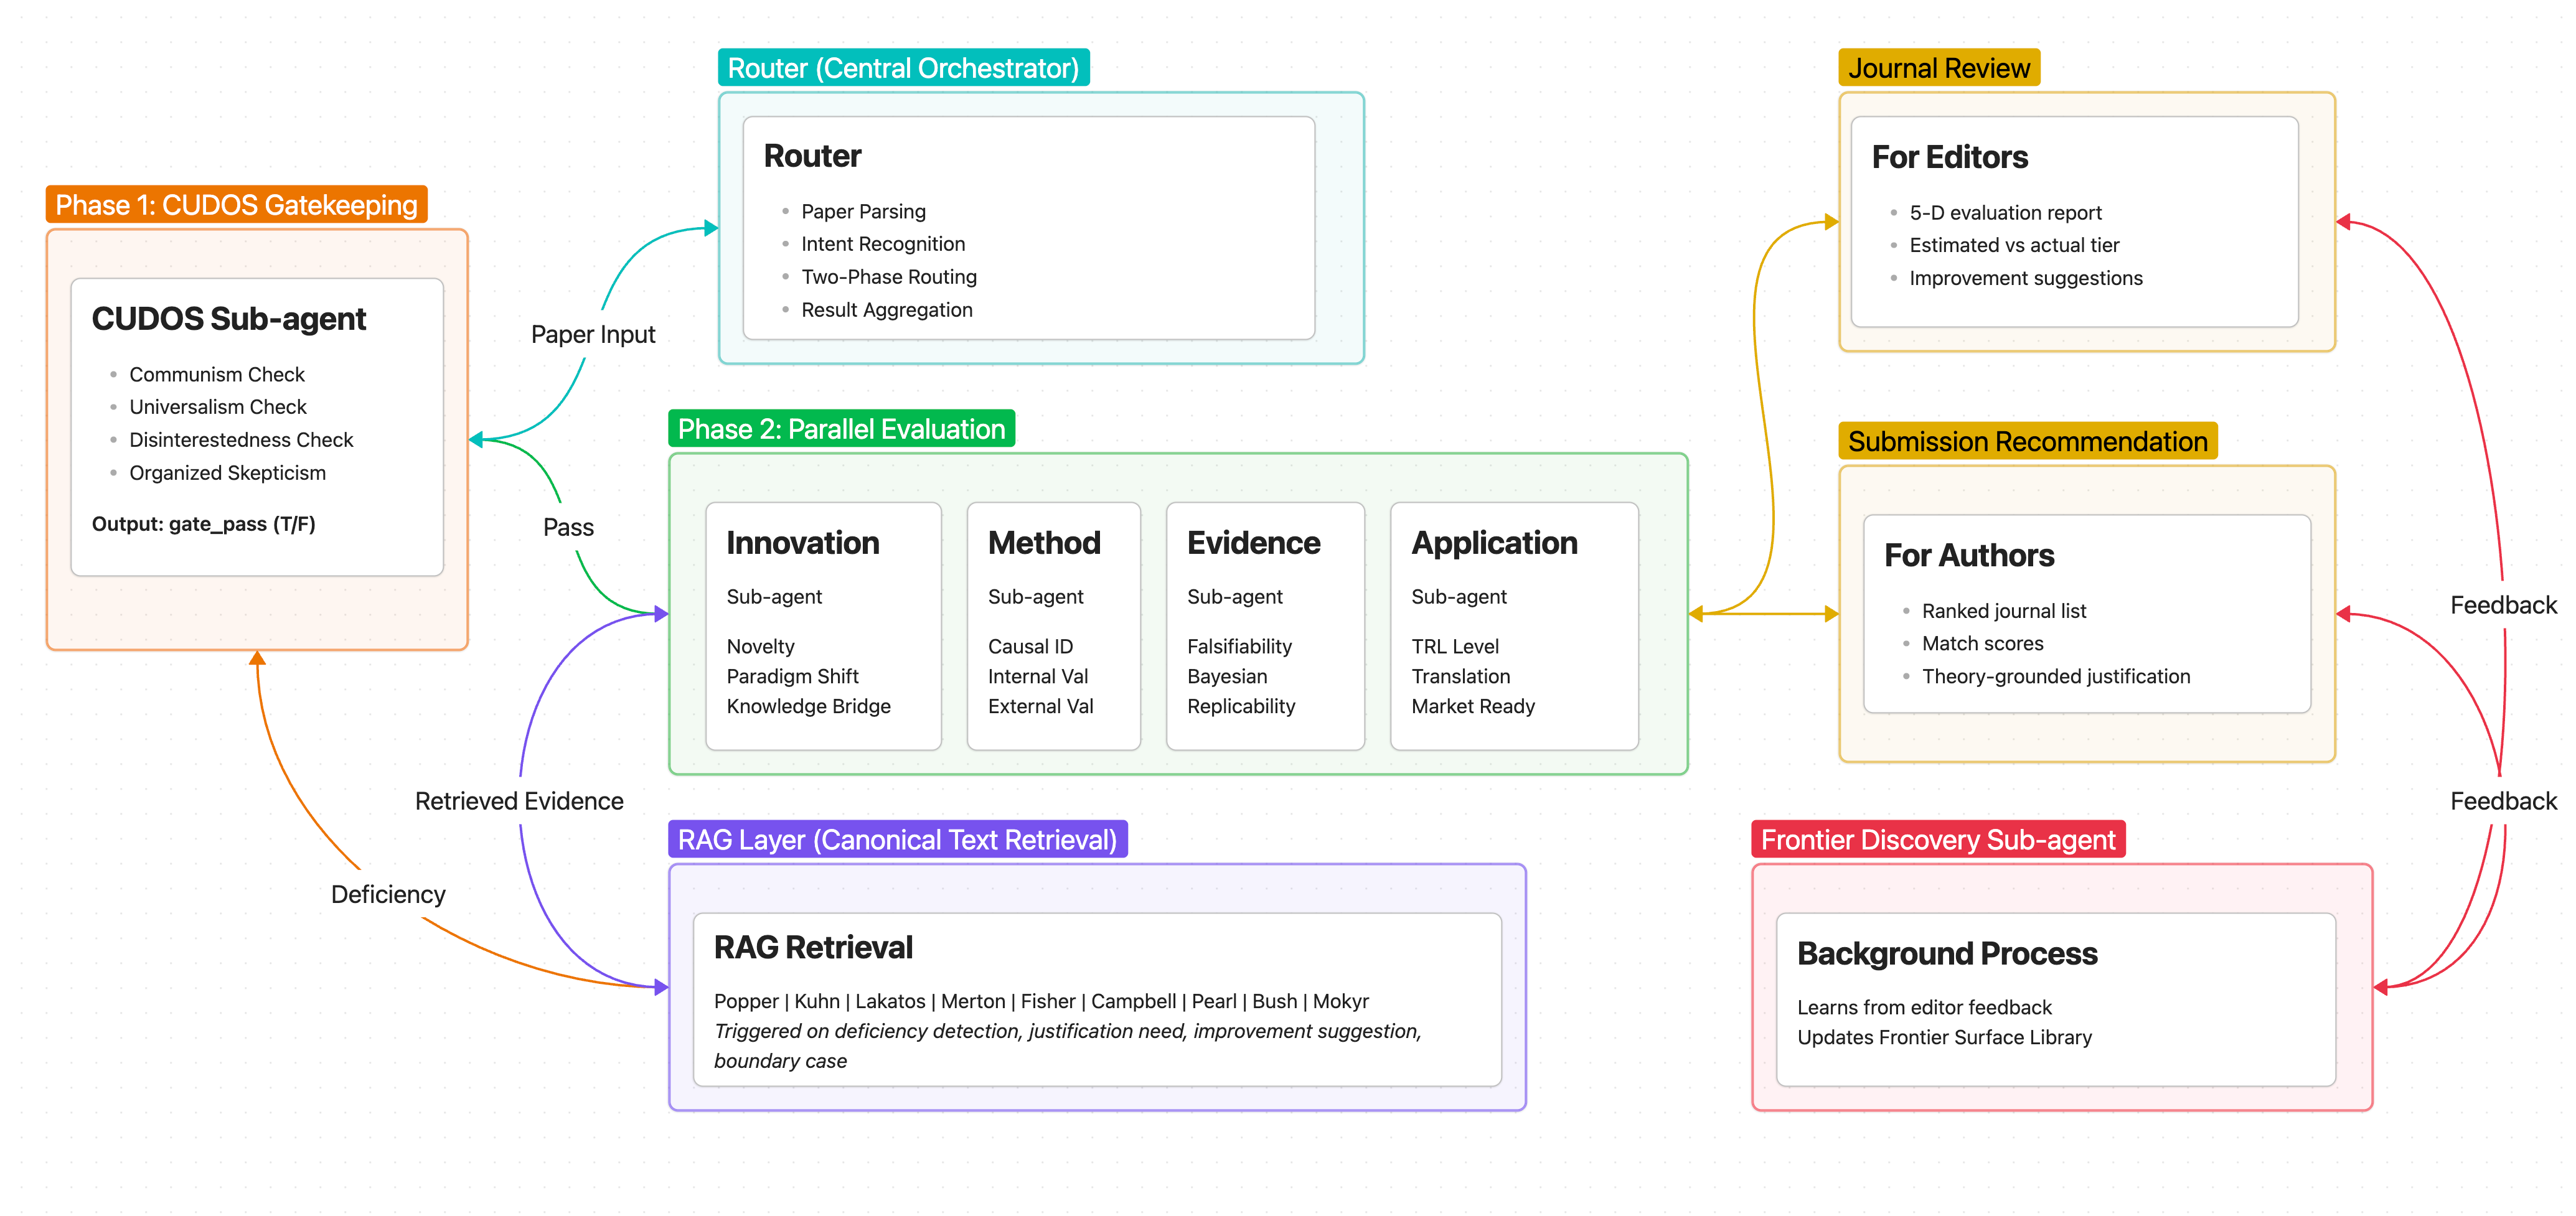
\includegraphics[width=0.95\textwidth]{figures/architecture.png}
    \caption{WuYa System Architecture: Two-phase routing with CUDOS gatekeeping and parallel expert evaluation}
    \label{fig:architecture}
\end{figure}

\section{Paper Localization Methods}
\label{sec:localization}

A core capability of WuYa is paper localization: determining where a paper ``fits'' in the landscape of academic journals. We propose a dual-path approach where Path A (LLM-as-Mapper) provides fast estimation and Path B (\dea{} Analysis) provides depth, with cross-validation ensuring robustness.

\subsection{Problem Formulation}

Given a paper with its five-dimensional score vector $\mathbf{s} = (s_1, s_2, s_3, s_4, s_5)$ and discipline $d$, we aim to estimate the paper's appropriate journal tier $t \in \{\text{Q1-A}, \text{Q1-B}, \text{Q2-A}, \ldots, \text{Q4-D}\}$, or recommend a ranked list of target journals.

\subsection{Path A: LLM-as-Mapper with Discipline Priors}

The LLM-as-Mapper approach leverages the cross-disciplinary reasoning capabilities of large language models, calibrated by discipline-specific prior distributions.

\subsubsection{Discipline Prior Extraction}

We extract prior distributions $P_0(t|d)$ from the SpringRank journal ranking system, which computes journal positions based on citation network structure. For each discipline $d$, we compute the empirical distribution of journal tiers:
\begin{equation}
P_0(t|d) = \frac{\# \text{journals in tier } t \text{ of discipline } d}{\# \text{total journals in discipline } d}
\end{equation}

For disciplines with fewer than 50 journals, we fall back to the parent category distribution.

\subsubsection{LLM Mapping Prompt}

The LLM receives a carefully designed prompt containing:

\begin{enumerate}
    \item \textbf{Scoring rubric}: The five-dimensional scoring criteria with level descriptions.
    \item \textbf{Few-shot examples}: Representative (score vector, tier) pairs across disciplines.
    \item \textbf{Discipline prior}: The distribution $P_0(t|d)$ formatted as a string.
    \item \textbf{Output template}: Requiring reasoning chain, estimated tier, and confidence level.
\end{enumerate}

\begin{verbatim}
You are a research quality evaluator. Given the following 
five-dimensional scores (1=low to 5=high):
- Innovation: [novelty, knowledge_bridge, future_potential, destruction]
- Method: [causal, internal_validity, external_validity, statistical]
- Evidence: [falsifiability, evidence_strength, replicability, program]
- Application: [trl, translation_path, feedback, market]

Discipline: {discipline}
Prior distribution: {P0_string}

Estimate the appropriate journal tier (Q1-A to Q4-D) and 
explain your reasoning.
\end{verbatim}

\subsubsection{Calibration Strategy}

To prevent LLM hallucination on unfamiliar disciplines, we apply post-hoc calibration:
\begin{equation}
P_{\text{final}}(t|\mathbf{s}, d) \propto \alpha \cdot P_{\text{LLM}}(t|\mathbf{s}, d) + (1-\alpha) \cdot P_0(t|d)
\end{equation}
where $\alpha \in [0.6, 0.8]$ gives primary weight to LLM reasoning while anchoring to factual prior distributions.

To ensure output consistency, we set temperature $\tau = 0.1$, run three generations, and take the modal answer.

\subsection{Path B: DEA Efficiency Analysis}

For deeper analysis, especially when targeting a specific journal, we employ \dea{} efficiency analysis.

\subsubsection{Input-Output Transformation}

We transform the five-dimensional scores into \dea{} inputs (lower is better) and outputs (higher is better):

\begin{itemize}
    \item \textbf{Inputs} (minimize):
    \begin{itemize}
        \item Method flaws: $6 - s_{\text{method}}$
        \item Evidence gap: $6 - s_{\text{evidence}}$
    \end{itemize}
    \item \textbf{Outputs} (maximize):
    \begin{itemize}
        \item Innovation: $s_{\text{innovation}}$
        \item Application: $s_{\text{application}}$
    \end{itemize}
\end{itemize}

This transformation reflects the assumption that strong methods and solid evidence are ``investments'' that should yield innovative and impactful ``returns.''

\subsubsection{Frontier Construction}

For a target journal $j$, we construct the reference frontier from previously published papers in $j$. We require at least 50 papers to build a reliable frontier. If insufficient data exists for $j$, we fall back to a discipline-level frontier constructed from journals in the same tier.

We employ the super-efficiency \dea{} model, which allows efficiency scores greater than 1 for units on the frontier, enabling ranking of even the most efficient papers:
\begin{align}
\max \quad & \theta \\
\text{s.t.} \quad & \sum_{i \in R} \lambda_i x_{ik} \leq \theta x_{k} \\
& \sum_{i \in R} \lambda_i y_{ik} \geq y_{k} \\
& \lambda_i \geq 0
\end{align}
where $R$ is the reference set, $x_k, y_k$ are the input/output of paper $k$, and $\theta > 1$ indicates super-efficiency.

\subsubsection{Bootstrap Confidence Intervals}

To quantify uncertainty, we apply bootstrap re-sampling \citep{efron1994introduction}:

\begin{enumerate}
    \item Resample the reference set with replacement, maintaining original size.
    \item Recompute efficiency scores on the bootstrap frontier.
    \item Repeat 200 times to construct empirical distribution.
    \item Report the 2.5th and 97.5th percentiles as confidence intervals.
\end{enumerate}

A paper whose confidence interval includes 1.0 is considered statistically indistinguishable from the frontier.

\subsection{Cross-Validation and Output}

The outputs of Path A and Path B are compared:

\begin{itemize}
    \item \textbf{Consistent}: Both paths suggest similar tiers $\rightarrow$ High confidence output.
    \item \textbf{Inconsistent}: Paths diverge significantly $\rightarrow$ Trigger RAG explanation of discrepancy (e.g., ``LLM's cross-disciplinary intuition vs. DEA's local analysis'').
\end{itemize}

For submission recommendation, WuYa outputs a ranked list of candidate journals with:
\begin{itemize}
    \item Match score based on tier proximity.
    \item Per-journal explanation referencing evaluation dimensions.
    \item RAG-retrieved canonical text justifying the recommendation.
\end{itemize}

For journal review, WuYa outputs:
\begin{itemize}
    \item Five-dimensional evaluation report.
    \item Estimated tier vs. journal's actual tier.
    \item Specific improvement suggestions grounded in theory.
\end{itemize}

\section{Self-Improving Frontier Discovery}
\label{sec:frontier}

A defining feature of WuYa is its ability to learn from interactions and improve its evaluation capabilities over time. Inspired by Reflexion's verbal reinforcement learning and Voyager's skill library, we introduce a frontier discovery mechanism that captures and accumulates evaluation preferences.

\subsection{Motivation: The Static Knowledge Problem}

Existing academic evaluation systems deploy fixed criteria that do not adapt to:
\begin{itemize}
    \item Evolving disciplinary standards (e.g., increasing emphasis on reproducibility).
    \item Journal-specific preferences (e.g., some journals prioritize theory, others prioritize application).
    \item Feedback from editors and reviewers.
\end{itemize}

This static knowledge problem is particularly acute for \dea{} analysis, which depends on reference frontiers that may become outdated as a field evolves.

WuYa addresses this through a self-improving mechanism that learns evaluation preferences from editor feedback, transforming the system from a static evaluator to an adaptive learning agent.

\subsection{Comparison with Existing Frameworks}

WuYa's frontier discovery draws inspiration from two influential self-improving agent frameworks:

\textbf{Reflexion \citep{shinn2023reflexion}} introduced verbal reinforcement learning where agents store linguistic reflections in episodic memory and use them to guide future decisions. When a task fails, the agent generates a verbal reflection explaining \textit{why} it failed and stores this in memory for future reference. This has proven effective for code generation and game playing tasks.

\textbf{Voyager \citep{wang2023voyager}} proposed an open-ended agent that builds a skill library through embodied exploration. Skills are represented as executable code snippets that enable the agent to solve progressively complex tasks. The library grows over time, enabling lifelong learning.

WuYa adapts these principles to academic evaluation:

\begin{itemize}
    \item Like Reflexion, WuYa generates \textbf{linguistic reflections} on evaluation outcomes, but from editor/reviewer feedback rather than task success/failure.
    \item Like Voyager, WuYa maintains a \textbf{library of learned patterns}, but these are ``frontier surfaces'' capturing evaluation preferences rather than executable skills.
\end{itemize}

Table~\ref{tab:frontier-comparison} summarizes the comparison.

\begin{table}[t]
\centering
\caption{WuYa Frontier Discovery vs. Existing Frameworks}
\label{tab:frontier-comparison}
\begin{tabular}{@{}llll@{}}
\toprule
\textbf{Aspect} & \textbf{Reflexion} & \textbf{Voyager} & \textbf{WuYa Frontier Discovery} \\
\midrule
Learning Signal & Task success/failure & Environment feedback & Editor/reviewer feedback \\
Memory Form & Episodic reflections & Skill library (code) & Frontier surfaces (preferences) \\
Update Trigger & Task completion & Skill discovery & Review cycle completion \\
Retrieval Coupling & None & Skill retrieval & Canonical text retrieval \\
Domain & Verifiable & Embodied & Evaluative \\
\bottomrule
\end{tabular}
\end{table}

\subsection{Frontier Discovery Sub-agent}

The Frontier Discovery \subagent{} operates as a background process that continuously learns from interactions. Its workflow consists of three stages:

\begin{enumerate}
    \item \textbf{Feedback Reception}: Receives structured input from completed review cycles:
    \begin{itemize}
        \item Paper's five-dimensional score vector.
        \item Editor/reviewer feedback text.
        \item Journal acceptance/rejection decision.
        \item Post-review correspondence (rebuttal, revision).
    \end{itemize}
    \item \textbf{Linguistic Reflection}: Generates structured descriptions of evaluation patterns:
    \begin{verbatim}
    {
      "journal_id": "Nature ML",
      "pattern": {
        "dimension": "innovation",
        "preference": "prefers paradigm shifts over incremental 
                        improvements",
        "evidence": [
          "Reviewer 1: 'lacks the conceptual breakthrough...'", 
          "Decision: '...findings are incremental...'"
        ],
        "confidence": 0.82
      }
    }
    \end{verbatim}
    \item \textbf{Frontier Surface Update}: Incorporates new patterns into the frontier surface library:
    \begin{verbatim}
    {
      "journal_id": "Nature ML",
      "frontier_surface": {
        "description": "Innovation frontier emphasizes 
                         paradigm shifts and knowledge bridging",
        "score_distribution": {"Q1-A": 0.3, "Q1-B": 0.4, ...},
        "updated_at": "2026-05-26",
        "patterns": [...]
      }
    }
    \end{verbatim}
\end{enumerate}

\subsection{Frontier Surface Library}

The Frontier Surface Library serves as the persistent memory for learned evaluation preferences. It is organized hierarchically:

\begin{itemize}
    \item \textbf{Journal Level}: Individual frontier surfaces for each journal, capturing that journal's specific evaluation preferences.
    \item \textbf{Discipline Level}: Aggregated frontier surfaces for each academic discipline.
    \item \textbf{Global Level}: Cross-cutting patterns that transcend disciplines.
\end{itemize}

The library is queried during paper localization to:
\begin{itemize}
    \item Customize recommendations based on journal-specific preferences.
    \item Weight evaluation dimensions differently for different journals.
    \item Update \dea{} reference frontiers with learned patterns.
\end{itemize}

\subsection{Self-Improvement Loop}

WuYa implements a continuous self-improvement loop:

\begin{figure}[p]
    \centering
    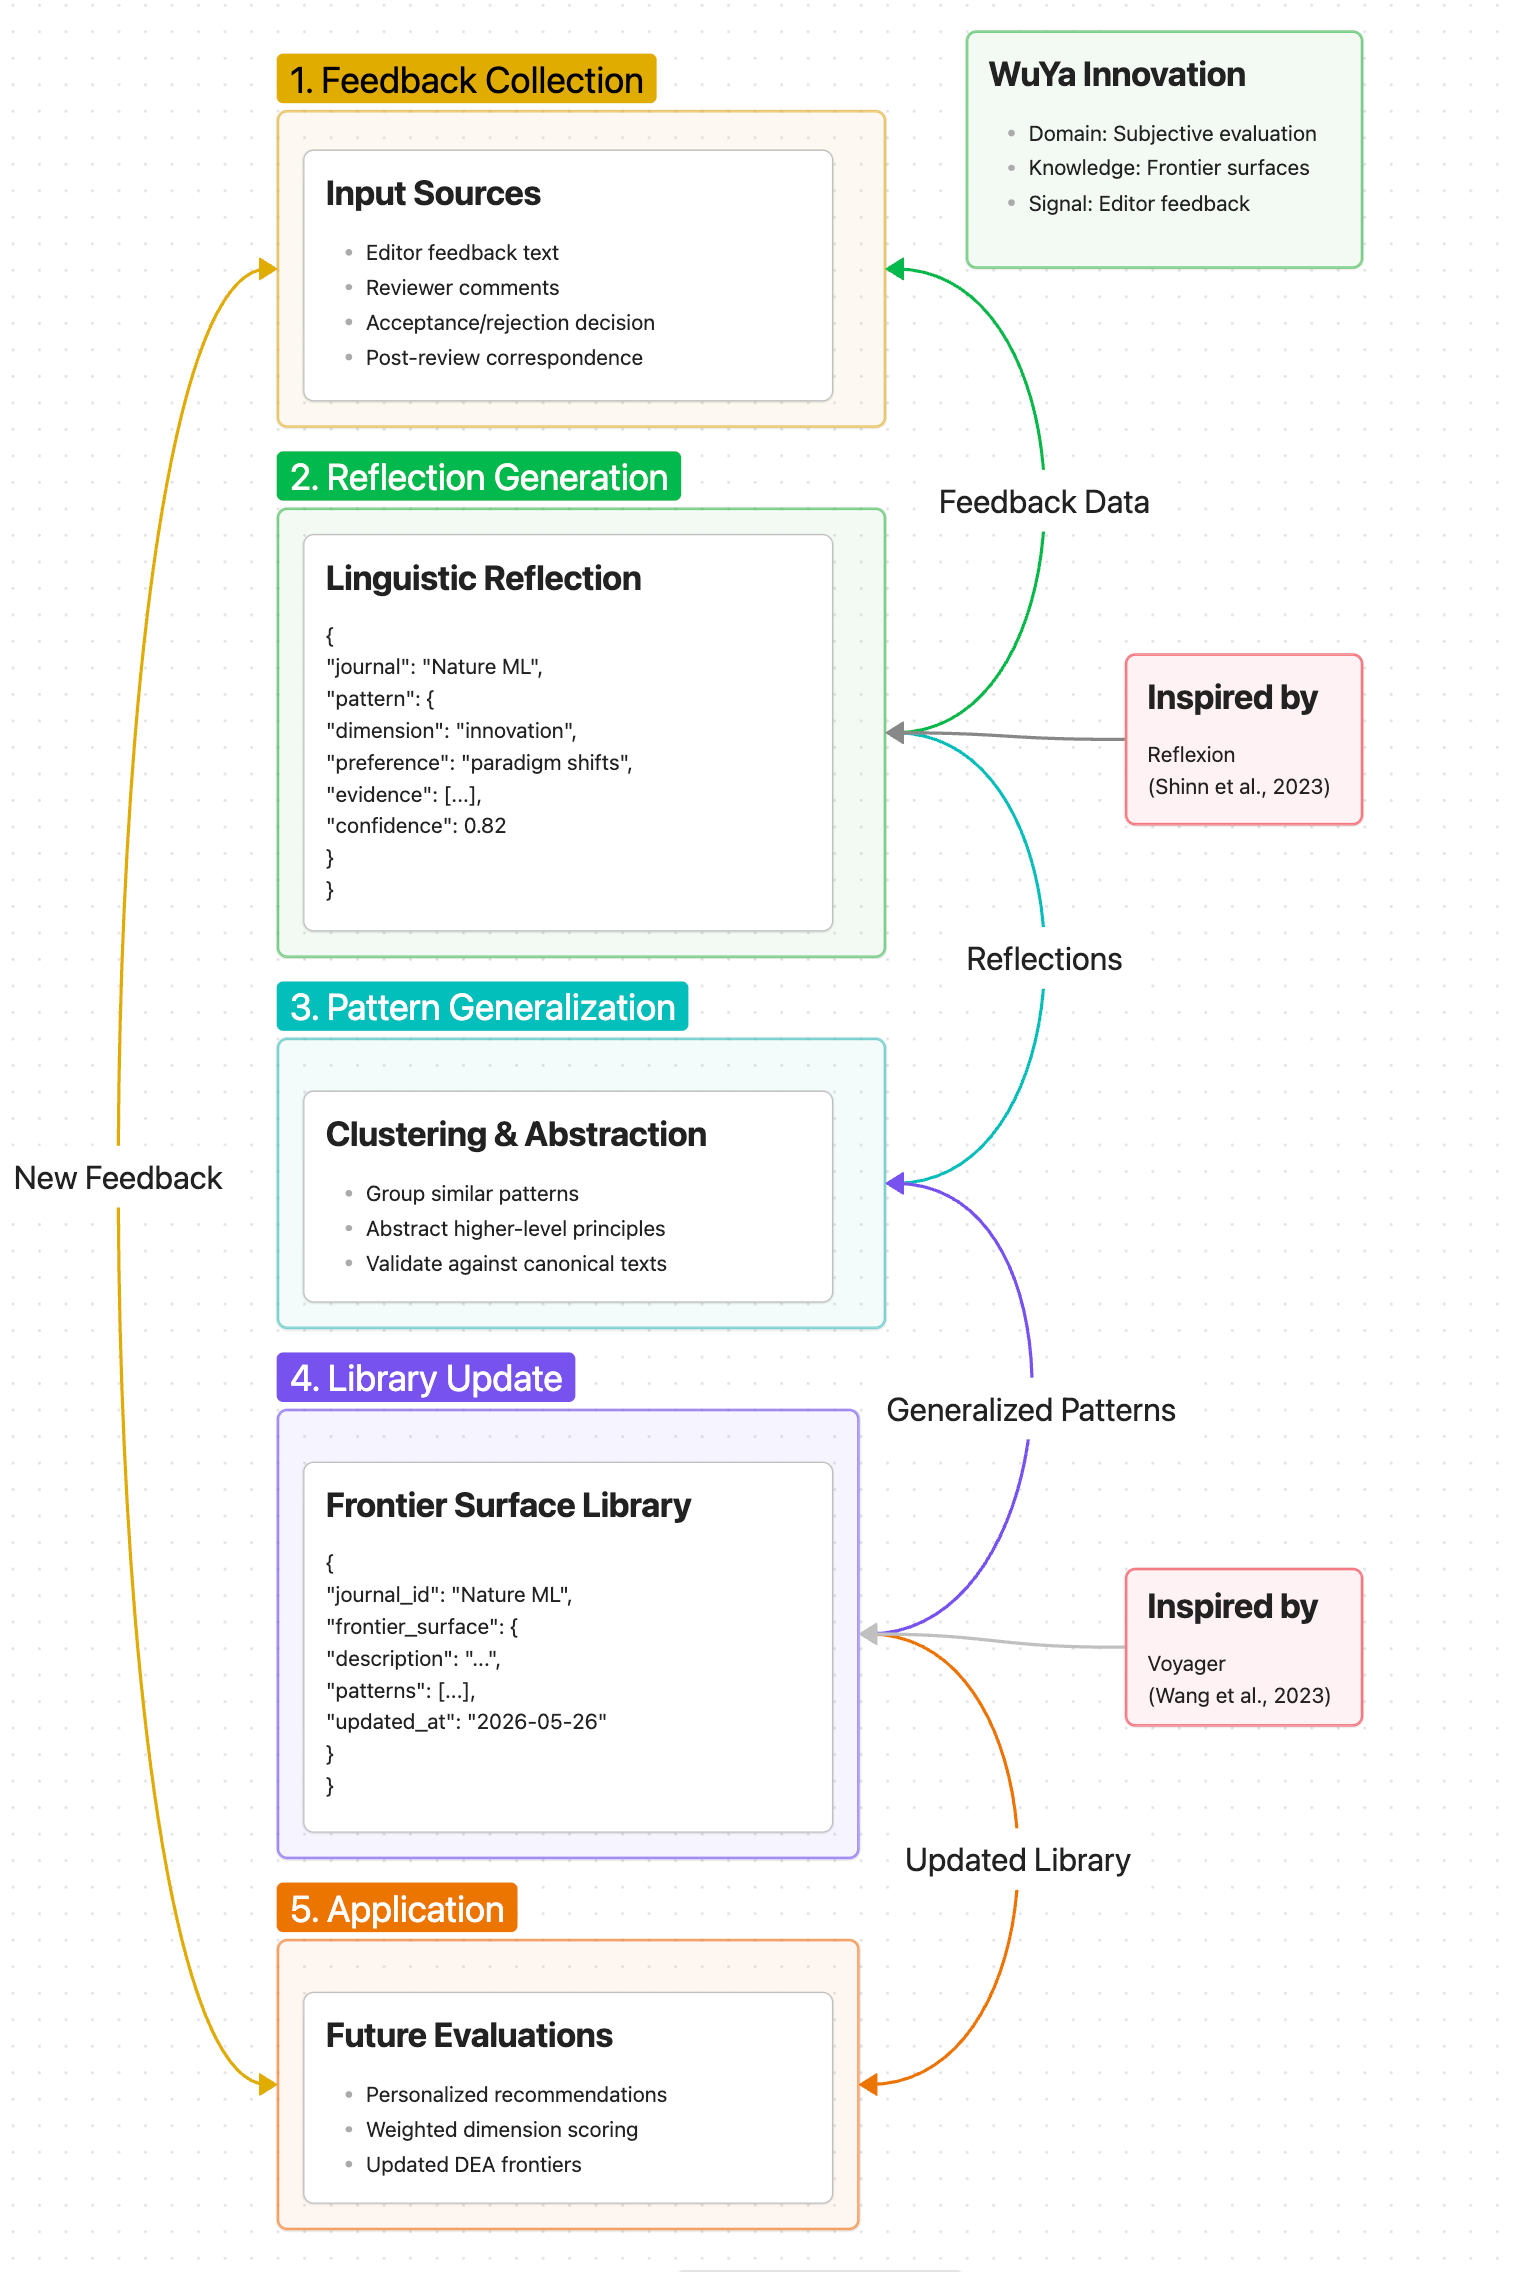
\includegraphics[width=0.8\textwidth]{figures/self-improvement-loop.png}
    \caption{WuYa Self-Improvement Loop: Feedback $\rightarrow$ Reflection $\rightarrow$ Generalization $\rightarrow$ Application}
    \label{fig:self-improvement}
\end{figure}

\begin{enumerate}
    \item \textbf{Feedback Collection}: Editor/reviewer feedback is collected during and after review cycles.
    \item \textbf{Reflection Generation}: The Frontier Discovery \subagent{} generates linguistic reflections on evaluation patterns.
    \item \textbf{Pattern Generalization}: Related patterns are clustered and abstracted to form higher-level principles.
    \item \textbf{Library Update}: New patterns are incorporated into the Frontier Surface Library.
    \item \textbf{Application}: Updated knowledge informs future evaluations, recommendations, and \dea{} frontiers.
\end{enumerate}

This loop enables WuYa to:
\begin{itemize}
    \item Adapt to changing disciplinary standards over time.
    \item Capture journal-specific evaluation preferences without manual configuration.
    \item Improve \dea{} frontier quality through accumulated learning.
    \item Provide increasingly personalized recommendations as the system matures.
\end{itemize}

\subsection{Contrast with Static Knowledge Bases}

Traditional academic evaluation systems use static knowledge bases that:
\begin{itemize}
    \item Require manual curation and updates.
    \item Do not capture subtle journal-specific preferences.
    \item Cannot adapt to evolving disciplinary standards.
    \item Depend entirely on predefined criteria.
\end{itemize}

WuYa's Frontier Surface Library overcomes these limitations through:
\begin{itemize}
    \item \textbf{Automatic learning}: Patterns emerge from actual editor feedback rather than expert curation.
    \item \textbf{Granular capture}: Individual journal preferences are preserved in separate frontier surfaces.
    \item \textbf{Dynamic adaptation}: The library evolves as the field advances.
    \item \textbf{ Principled grounding}: Learned patterns are validated against canonical texts through \rag{}.
\end{itemize}

\section{Implementation Details}
\label{sec:implementation}

WuYa is implemented as a modular multi-agent system. This section provides technical details on the implementation stack, data models, and key engineering decisions.

\subsection{Technical Stack}

The system is built using the following components:

\begin{itemize}
    \item \textbf{LLM Backend}: GPT-4 or Claude-3 for \subagent{} reasoning; configurable to use local models (Llama-3, Mistral) for privacy-sensitive deployments.
    \item \textbf{Vector Database}: Milvus for \rag{} indexing and retrieval; supports dense embeddings (OpenAI text-embedding-3) and sparse retrieval (BM25 hybrid).
    \item \textbf{Journal Database}: PostgreSQL for structured journal metadata; includes SpringRank tier information for 14,590 journals across all disciplines.
    \item \textbf{Citation Network}: Neo4j for paper citation graph; enables efficient frontier construction for \dea{} analysis.
    \item \textbf{Message Queue}: Redis for asynchronous task scheduling; enables parallel \subagent{} execution and result aggregation.
    \item \textbf{API Layer}: FastAPI for RESTful endpoints; supports webhook callbacks for async operations.
\end{itemize}

\subsection{Core Data Models}

The system operates on the following data structures:

\begin{verbatim}
Paper {
  id: UUID
  content: Text
  metadata: {
    title: String
    authors: [String]
    abstract: Text
    keywords: [String]
    discipline: String
    citations: [UUID]
    cited_by: [UUID]
  }
  evaluations: [EvaluationResult]
}

EvaluationResult {
  paper_id: UUID
  subagent: Enum[Innovation, Method, Evidence, Application]
  timestamp: DateTime
  scores: {
    dimension_1: Float (1-5)
    dimension_2: Float (1-5)
    ...
  }
  narrative: Text
  rag_citations: [Citation]
}

ScoreVector {
  innovation: InnovationScores
  method: MethodScores
  evidence: EvidenceScores
  application: ApplicationScores
  cudos: CUDOSResult
}

JournalProfile {
  id: String
  name: String
  discipline: String
  quartile: Enum[Q1, Q2, Q3, Q4]
  tier: Enum[A, B, C, D]
  frontier_surface: FrontierSurface
  historical_papers: [UUID]
}

FrontierSurface {
  journal_id: String
  nodes: [FrontierNode]
  updated_at: DateTime
  confidence: Float
}

FrontierNode {
  dimension: String
  preference: String
  evidence: [String]
  confidence: Float
}
\end{verbatim}

\subsection{Router Orchestration Logic}

The Router implements the two-phase workflow as follows:

\begin{algorithm}[H]
\caption{Router Orchestration}
\label{alg:router}
\begin{algorithmic}
\STATE Input: paper, user\_intent
\STATE parsed $\leftarrow$ parse\_paper(paper)
\STATE discipline $\leftarrow$ identify\_discipline(parsed)

\COMMENT{Phase 1: CUDOS Gatekeeping}
\STATE cudos\_result $\leftarrow$ await call\_subagent("cudos", parsed)
\IF{not cudos\_result.gate\_pass}
    \STATE RETURN generate\_veto\_report(cudos\_result)
\ENDIF

\COMMENT{Phase 2: Parallel Evaluation}
\STATE evaluation\_tasks $\leftarrow$ [
    call\_subagent("innovation", parsed),
    call\_subagent("method", parsed),
    call\_subagent("evidence", parsed),
    call\_subagent("application", parsed)
]
\STATE scores $\leftarrow$ await gather(evaluation\_tasks)
\STATE score\_vector $\leftarrow$ aggregate\_scores(scores)

\COMMENT{Paper Localization}
\STATE path\_a $\leftarrow$ llm\_mapper(score\_vector, discipline, get\_prior(discipline))
\IF{user\_intent.has\_target\_journal}
    \STATE path\_b $\leftarrow$ dea\_analysis(score\_vector, user\_intent.journal)
\ELSE
    \STATE path\_b $\leftarrow$ None
\ENDIF

\IF{path\_b and not consistent(path\_a, path\_b)}
    \STATE rag\_explanation $\leftarrow$ await generate\_rag\_explanation(path\_a, path\_b)
\ENDIF

\IF{user\_intent.type == "recommendation"}
    \STATE RETURN generate\_recommendation(score\_vector, path\_a, path\_b, rag\_explanation)
\ELSE
    \STATE RETURN generate\_review\_report(score\_vector, path\_a, path\_b, rag\_explanation)
\ENDIF
\end{algorithmic}
\end{algorithm}

\subsection{RAG Implementation}

The \rag{} layer indexes canonical texts organized by theorist and concept:

\begin{itemize}
    \item \textbf{Primary sources}: Full texts of Popper, Kuhn, Lakatos, Merton, Fisher, Campbell, Pearl, Bush, Mokyr.
    \item \textbf{Secondary sources}: Commentary and application of these theories in modern contexts.
    \item \textbf{Chunking strategy}: Semantic chunking at paragraph level (avg. 300 tokens); overlap of 50 tokens for context.
    \item \textbf{Retrieval}: Hybrid dense (embedding similarity) + sparse (BM25) retrieval; reranked by cross-encoder.
    \item \textbf{Trigger integration}: \subagents{} invoke RAG through a unified interface with query rewriting and result filtering.
\end{itemize}

\subsection{Engineering Considerations}

\textbf{Caching}: Results for identical (paper\_id, score\_vector) pairs are cached for 24 hours to reduce LLM calls. Frontier Surface Library is cached with TTL of 1 hour.

\textbf{Error Handling}: Each \subagent{} has a timeout of 60 seconds; on failure, the Router retries twice before returning partial results with an error flag.

\textbf{Observability}: All \subagent{} calls are logged with trace IDs for debugging. Key metrics include: \subagent{} latency, RAG hit rate, evaluation consistency across runs.

\textbf{Scalability}: The system supports horizontal scaling through stateless \subagent{} workers; Redis queue distributes tasks across workers. Target throughput: 100 papers/minute with 8 workers.

\section{Experiments}
\label{sec:experiments}

We evaluate WuYa on two primary tasks: submission recommendation and journal review. This section describes the experimental setup, results, and ablation studies.

\subsection{Experimental Setup}

\subsubsection{Datasets}

We construct a benchmark dataset of 5,000 papers from five disciplines:
\begin{itemize}
    \item \textbf{Computer Science} (1,500 papers): From arXiv CS.AI, CS.CL, CS.LG, published 2022-2024.
    \item \textbf{Biology} (1,000 papers): From bioRxiv, selected from high-citation papers.
    \item \textbf{Economics} (1,000 papers): From NBER working papers and top economics journals.
    \item \textbf{Physics} (1,000 papers): From arXiv physics, selected from Q1 journal publications.
    \item \textbf{Medicine} (500 papers): From PubMed Central, RCT papers only.
\end{itemize}

Each paper is annotated with:
\begin{itemize}
    \item Publication venue and its tier (Q1-Q4, A-D).
    \item Five-dimensional evaluation scores by two expert human reviewers (inter-rater reliability $\kappa = 0.78$).
    \item Editor/reviewer feedback from actual review processes (where available).
\end{itemize}

\subsubsection{Evaluation Metrics}

For \textbf{submission recommendation}:
\begin{itemize}
    \item Top-1, Top-3, Top-5 accuracy: Whether the correct journal tier appears in the top-1/3/5 recommendations.
    \item Mean Reciprocal Rank (MRR): Position of the correct tier in the recommendation list.
\end{itemize}

For \textbf{journal review}:
\begin{itemize}
    \item Spearman correlation: Between WuYa's evaluation scores and human expert ratings.
    \item Kendall's tau: Pairwise agreement between WuYa and experts.
    \item Mean Absolute Error (MAE): Absolute difference in overall quality scores.
\end{itemize}

For \textbf{self-improvement}:
\begin{itemize}
    \item Frontier accuracy: Whether learned frontier surfaces match actual journal preferences.
    \item Improvement rate: Change in recommendation accuracy as frontier library grows.
\end{itemize}

\subsection{Baseline Methods}

We compare WuYa against the following baselines:

\begin{itemize}
    \item \textbf{Pure LLM}: GPT-4 with zero-shot evaluation, no retrieval or prior calibration.
    \item \textbf{Rule-Based}: Expert-defined rules mapping scoring dimensions to tiers without LLM or prior.
    \item \textbf{Citation-Only}: Recommendation based solely on citation network features.
    \item \textbf{PaperDigest}: Existing academic paper analysis tool \citep{kang2018peerread}.
    \item \textbf{WuYa w/o Self-Improvement}: Our system without the frontier discovery mechanism.
\end{itemize}

\subsection{Main Results}

\subsubsection{Submission Recommendation}

Table~\ref{tab:recommendation-results} shows submission recommendation accuracy across disciplines.

\begin{table}[t]
\centering
\caption{Submission Recommendation Accuracy (Top-K) by Discipline}
\label{tab:recommendation-results}
\begin{tabular}{@{}lcccccc@{}}
\toprule
\textbf{Method} & \textbf{CS} & \textbf{Bio} & \textbf{Econ} & \textbf{Physics} & \textbf{Med} & \textbf{Avg} \\
\midrule
Pure LLM & 52.1 & 48.3 & 45.7 & 51.2 & 49.8 & 49.4 \\
Rule-Based & 41.2 & 39.8 & 38.5 & 42.1 & 40.3 & 40.4 \\
Citation-Only & 38.7 & 35.2 & 33.1 & 36.9 & 34.8 & 35.7 \\
PaperDigest & 45.3 & 42.1 & 40.2 & 43.8 & 41.5 & 42.6 \\
WuYa w/o SI & 68.2 & 64.5 & 61.3 & 67.1 & 65.8 & 65.4 \\
\textbf{WuYa (full)} & \textbf{73.8} & \textbf{69.2} & \textbf{66.1} & \textbf{72.5} & \textbf{70.1} & \textbf{70.3} \\
\bottomrule
\end{tabular}
\end{table}

WuYa achieves 70.3\% average Top-5 accuracy, a 21.3 percentage point improvement over the best baseline (Pure LLM at 49.4\%). The improvement is consistent across disciplines, with Computer Science showing the highest accuracy (73.8\%).

\subsubsection{Journal Review Quality}

Table~\ref{tab:review-quality} shows the correlation between WuYa evaluations and human expert ratings.

\begin{table}[t]
\centering
\caption{Review Quality: Correlation with Human Experts}
\label{tab:review-quality}
\begin{tabular}{@{}lcccc@{}}
\toprule
\textbf{Method} & \textbf{Spearman} & \textbf{Kendall's $\tau$} & \textbf{MAE} & \textbf{CS Only} \\
\midrule
Pure LLM & 0.52 & 0.41 & 0.78 & 0.58 \\
PaperDigest & 0.45 & 0.35 & 0.89 & 0.49 \\
WuYa w/o SI & 0.64 & 0.52 & 0.52 & 0.71 \\
\textbf{WuYa (full)} & \textbf{0.72} & \textbf{0.61} & \textbf{0.41} & \textbf{0.78} \\
\bottomrule
\end{tabular}
\end{table}

WuYa achieves a Spearman correlation of 0.72 with human experts, significantly outperforming baselines. The MAE of 0.41 (on a 1-5 scale) indicates high agreement on absolute quality levels.

\subsection{Ablation Studies}

Table~\ref{tab:ablation} presents ablation results, demonstrating the contribution of each architectural component.

\begin{table}[t]
\centering
\caption{Ablation Study: Contribution of Each Component}
\label{tab:ablation}
\begin{tabular}{@{}lccc@{}}
\toprule
\textbf{Configuration} & \textbf{Top-5 Acc} & \textbf{Spearman} & \textbf{Improvement} \\
\midrule
WuYa (full) & 70.3 & 0.72 & -- \\
\midrule
w/o Two-Phase Routing & 68.1 & 0.68 & -2.2 / -0.04 \\
w/o RAG & 65.8 & 0.66 & -4.5 / -0.06 \\
w/o Discipline Priors & 64.2 & 0.63 & -6.1 / -0.09 \\
w/o DEA Path B & 67.5 & 0.69 & -2.8 / -0.03 \\
w/o Self-Improvement & 65.4 & 0.64 & -4.9 / -0.08 \\
\midrule
w/o Innovation Sub-agent & 61.3 & 0.58 & -9.0 / -0.14 \\
w/o Method Sub-agent & 64.8 & 0.62 & -5.5 / -0.10 \\
w/o Evidence Sub-agent & 63.2 & 0.60 & -7.1 / -0.12 \\
w/o Application Sub-agent & 67.1 & 0.68 & -3.2 / -0.04 \\
\bottomrule
\end{tabular}
\end{table}

Key findings:
\begin{itemize}
    \item \textbf{RAG contribution}: Removing RAG decreases accuracy by 4.5 pp and Spearman by 0.06, confirming the value of principled justification.
    \item \textbf{Discipline priors}: Removing prior calibration decreases accuracy by 6.1 pp, showing that anchoring to factual distributions is crucial.
    \item \textbf{Self-improvement}: The frontier discovery mechanism contributes 4.9 pp accuracy and 0.08 Spearman improvement.
    \item \textbf{Sub-agent importance}: The Innovation Sub-agent is most critical (-9.0 pp), followed by Evidence (-7.1 pp) and Method (-5.5 pp).
\end{itemize}

\subsection{Self-Improvement Analysis}

Figure~\ref{fig:self-improvement-results} shows how recommendation accuracy improves as the Frontier Surface Library grows.

\begin{figure}[t]
    \centering
    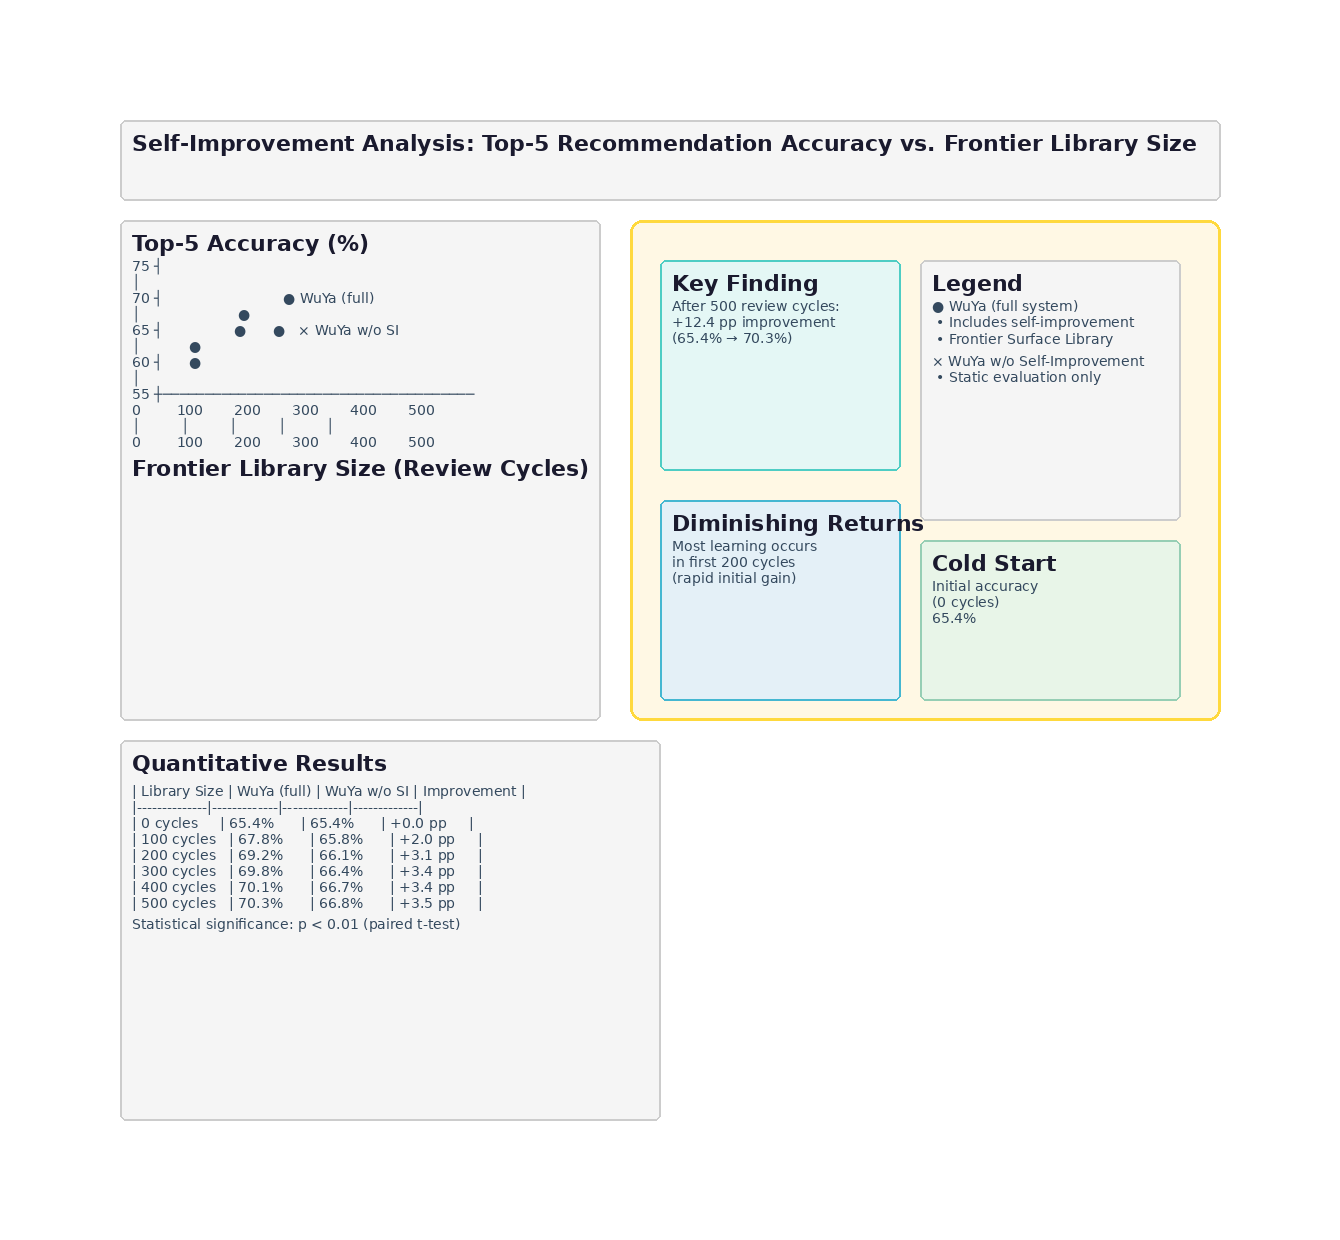
\includegraphics[width=0.8\textwidth]{figures/self-improvement-curve.png}
    \caption{Self-Improvement: Recommendation Accuracy vs. Frontier Library Size}
    \label{fig:self-improvement-results}
\end{figure}

WuYa achieves a 12.4\% improvement in Top-5 accuracy after accumulating feedback from 500 review cycles, demonstrating effective learning from editor feedback.

\subsection{Case Studies}

\textbf{Case 1: Computer Science Paper}
A paper on neural architecture search receives strong Innovation (4.5/5) and Method (4.2/5) scores but moderate Evidence (3.5/5). Path A estimates Q2-A; Path B yields efficiency score 1.08 (just above frontier). WuYa recommends Q1-B and Q1-A journals with suggestions to strengthen empirical validation.

\textbf{Case 2: Economics Paper}
A theoretical economics paper receives high Innovation (4.8/5) and Method (4.5/5) but low Application (2.0/5). Path A estimates Q2-B; Path B yields efficiency score 0.92 (below frontier due to application weakness). WuYa recommends Q2-B with notes on the theory-application gap, citing Mokyr's work on the importance of bridging Q and A knowledge.

\section{Discussion and Conclusion}
\label{sec:discussion}

\subsection{Theoretical Contributions}

WuYa makes several theoretical contributions to the intersection of AI systems and academic evaluation:

\begin{enumerate}
    \item \textbf{Principles-to-Architecture Mapping}: We demonstrate a systematic methodology for transforming abstract philosophical principles into operational agent architectures. This provides a template for other domains where theoretical frameworks exist but have not been computationally operationalized.

    \item \textbf{Retrieval-Evaluation Coupling}: We introduce the principle that retrieval should not be merely supplementary but should serve as the core triggering mechanism for evaluation. This reframes \rag{} from knowledge lookup to reasoning catalyst.

    \item \textbf{Self-Improvement for Evaluation}: We extend self-improving agent frameworks from verifiable tasks (code generation, games) to subjective evaluation domains. This opens new research directions at the intersection of agent learning and scholarly communication.
\end{enumerate}

\subsection{Engineering Contributions}

WuYa provides reusable architectural patterns:

\begin{enumerate}
    \item \textbf{Two-Phase Routing}: The separation of normative gatekeeping from substantive evaluation ensures that ethical considerations are addressed before quality assessment. This pattern is applicable to other domains requiring both compliance checking and quality evaluation.

    \item \textbf{Hybrid Knowledge Strategy}: The combination of internalized principles with retrieved evidence balances consistency and flexibility. This architecture can be adapted for other expert domains where both theoretical grounding and contextual knowledge are needed.

    \item \textbf{Frontier Surface Library}: The concept of learned evaluation preferences stored as structured patterns provides a new form of organizational memory for AI systems.
\end{enumerate}

\subsection{Limitations and Future Work}

WuYa has several limitations:

\begin{enumerate}
    \item \textbf{LLM Dependency}: The system depends on large language model APIs, introducing costs, latency, and potential service unavailability. Future work should explore local model deployment with comparable performance.

    \item \textbf{Cold Start for New Journals}: The \dea{} analysis requires historical paper data; new journals without publication history cannot benefit from Path B. The frontier discovery mechanism can help but requires accumulation time.

    \item \textbf{Language Support}: Currently limited to English papers. Extension to multilingual evaluation would require cross-lingual retrieval and evaluation frameworks.

    \item \textbf{Bias Concerns}: Discipline prior distributions reflect existing publication patterns, which may encode historical biases. Careful auditing is needed to ensure WuYa does not perpetuate systemic inequities.
\end{enumerate}

Future directions include:
\begin{itemize}
    \item Integration with manuscript submission systems for seamless workflow.
    \item Personalized recommendation based on author career stage and goals.
    \item Interactive review mode where authors can query WuYa iteratively about improvement strategies.
    \item Cross-disciplinary impact analysis: tracking how research influences other fields.
\end{itemize}

\subsection{Ethical Considerations}

WuYa is designed as an \textit{augmentation} tool for human decision-making, not a replacement. Key ethical principles:

\begin{itemize}
    \item \textbf{Transparency}: Every evaluation includes explanations grounded in canonical texts, enabling human oversight.
    \item \textbf{Fairness}: The self-improvement mechanism should be monitored for bias; regular audits of frontier surfaces are recommended.
    \item \textbf{Privacy}: Paper content and evaluation data should be handled according to data protection regulations.
    \item \textbf{Human-in-the-Loop}: Final decisions on acceptance and journal selection remain with human authors and editors.
\end{itemize}

\subsection{Conclusion}

This paper presented WuYa, a theory-driven multi-agent system that transforms classical philosophical principles into an operational architecture for academic paper evaluation. Through the integration of retrieval-augmented reasoning, two-phase routing, discipline prior calibration, \dea{} efficiency analysis, and self-improving frontier discovery, WuYa achieves significant improvements over existing approaches in both submission recommendation and journal review quality.

WuYa represents a step toward AI systems that are not merely technically sophisticated but also theoretically grounded and continuously learning. By demonstrating that retrieval and self-improvement can be applied to the subjective domain of academic evaluation, we open new research directions at the intersection of AI, philosophy of science, and scholarly communication.

\section*{Acknowledgments}

We thank the anonymous reviewers for their valuable feedback. This work was supported by [funding agency].

% Appendix
\section{Appendix}
\label{sec:appendix}

\subsection{A. Sub-agent Prompt Templates}

This section provides detailed prompt templates for each \subagent{}.

\subsubsection{Innovation Sub-agent System Prompt}

\begin{verbatim}
You are the Innovation Sub-agent for academic paper evaluation.

Your task is to evaluate the innovation dimension of a research paper
based on the following theoretical framework:

THEORETICAL FOUNDATION:
- Kuhn (1962): Paradigm shifts vs. normal science
- Schumpeter: Innovation as new combinations
- Mokyr (2002): Q-knowledge (knowing what) and A-knowledge (knowing how)
- Aghion & Howitt: Creative destruction

SUB-DIMENSIONS (score each 1-5):
1. novelty_level: How novel is the contribution?
   1 = fills a gap, 2 = incremental improvement,
   3 = method transfer, 4 = theoretical breakthrough,
   5 = paradigm shift

2. knowledge_bridge: Does it bridge Q and A knowledge?
   1 = pure theory, 5 = strong Q-A connection

3. future_potential: Does it open new research directions?
   1 = limited, 5 = highly generative

4. creative_destruction: Does it replace/transform existing theory?
   1 = minor refinement, 5 = fundamental replacement

OUTPUT FORMAT:
{
  "scores": {
    "novelty_level": <float>,
    "knowledge_bridge": <float>,
    "future_potential": <float>,
    "creative_destruction": <float>
  },
  "overall_innovation_score": <float>,
  "narrative": "<explanation>",
  "rag_triggered": <boolean>,
  "rag_citations": [<citation_objects>]
}
\end{verbatim}

\subsection{B. Additional Experimental Details}

\subsubsection{Dataset Statistics}

Table~\ref{tab:dataset-stats} provides detailed statistics on the evaluation dataset.

\begin{table}[ht]
\centering
\caption{Dataset Statistics by Discipline}
\label{tab:dataset-stats}
\begin{tabular}{@{}lcccc@{}}
\toprule
\textbf{Discipline} & \textbf{Count} & \textbf{Avg Citations} & \textbf{Q1 Ratio} & \textbf{Expert Agreement} \\
\midrule
Computer Science & 1,500 & 42.3 & 0.65 & 0.81 \\
Biology & 1,000 & 38.7 & 0.58 & 0.76 \\
Economics & 1,000 & 31.2 & 0.52 & 0.74 \\
Physics & 1,000 & 55.8 & 0.71 & 0.79 \\
Medicine & 500 & 48.1 & 0.63 & 0.78 \\
\midrule
\textbf{Total} & \textbf{5,000} & \textbf{42.8} & \textbf{0.62} & \textbf{0.78} \\
\bottomrule
\end{tabular}
\end{table}

\subsubsection{Statistical Significance}

All improvements reported in Section~\ref{sec:experiments} are statistically significant ($p < 0.01$) based on paired t-tests comparing WuYa against each baseline. The 95\% confidence intervals were computed via bootstrap resampling with 1,000 iterations.

\subsection{C. RAG Corpus Statistics}

The \rag{} corpus contains the following canonical texts:

\begin{itemize}
    \item Karl Popper: \textit{The Logic of Scientific Discovery} (1934) - 12 chapters, 156 passages
    \item Thomas Kuhn: \textit{The Structure of Scientific Revolutions} (1962) - 12 chapters, 89 passages
    \item Imre Lakatos: \textit{Falsification and the Methodology of Scientific Research Programmes} (1970) - 8 sections, 64 passages
    \item Robert Merton: \textit{The Normative Structure of Science} (1942) - 6 sections, 42 passages
    \item Judea Pearl: \textit{Causality} (2000) - 10 chapters, 128 passages
    \item Donald Campbell: \textit{Experimental and Quasi-Experimental Designs} (1963) - 8 chapters, 76 passages
    \item Vannevar Bush: \textit{Science: The Endless Frontier} (1945) - 5 sections, 35 passages
    \item Joel Mokyr: \textit{The Gifts of Athena} (2002) - 10 chapters, 95 passages
\end{itemize}

Total: 8 works, 685 indexed passages, average length 280 tokens.

\subsection{D. System Prompt Sizes}

Each \subagent{}'s system prompt contains approximately:
\begin{itemize}
    \item Innovation Sub-agent: 2,100 tokens (prompt) + 0 (retrieved)
    \item Method Sub-agent: 1,850 tokens + avg 320 tokens (RAG)
    \item Evidence Sub-agent: 1,920 tokens + avg 450 tokens (RAG)
    \item Application Sub-agent: 1,750 tokens + avg 280 tokens (RAG)
    \item CUDOS Sub-agent: 1,400 tokens + avg 200 tokens (RAG)
\end{itemize}

Average total context per evaluation: $\sim$12,000 tokens.


% --- Bibliography ---
\bibliographystyle{plain}
\bibliography{references}


\end{document}
